\documentclass{fhnwreport} %
\usepackage[ngerman]{babel}
\usepackage[T1]{fontenc}
\usepackage[utf8]{inputenc}
\usepackage{tikz}
\usepackage{amsmath}
\usetikzlibrary{arrows}
\usepackage{lmodern}      % Type1-Schriftart für nicht-englische Texte 

%%% Harvard-Style Bibliographie
%\usepackage{natbib}
%\bibliographystyle{agsm}

%%% IEEE-Style Bibliographie
\bibliographystyle{IEEEtran}

%% Und wenn die Bibliographie im Inhaltsverzeichnis sein soll:
\usepackage[nottoc]{tocbibind}


\title{%
  Labor-Bericht\\[2ex]
  Simulink-Simulation eines PID-kontrollierten Gleichstrommotors}
\author{%
  Noah Hüsser und Almar Suter}

\begin{document}

% Titel
\maketitle

\tableofcontents

\section{Motivation}

Einen Regelkreis zu simulieren ist ein sehr interessanter Anwendungsfall für Matlab.
In diesem Versuch ging es insbesondere darum zwei physikalische Systeme in Simscape zu überbrücken und gemeinsam zu verwenden.
Dazu wurde die Regelung eines Elektromotors gewählt.

Im Abbildung \ref{fig:total} kann man den Regelkreis vom Aufbau her erkennen. Ziel ist es, dass eine gewünschte Drehzahl für einen Elektromotor eingestellt werden kann und der PID-Regler dafür sorgt, dass dieser Fall auch eintritt.
Da der Motor natürlich nur begrenzt Kraft hat und der Regler nicht perfekt ausregeln kann wird das Verhalten untersucht wenn am Motor eine Last angehängt wird (Schritt-Antwort).

Das Ziel dieses Versuches ist es einen Gleichstrommotor mit angeschlossener last durch einen PID-Regler zu regeln.

\section{Simulation}

Zu Anfang wurde ein einfacher Antrieb für den Motor wie in Abbildung \ref{fig:circuit_simple} TODO: gezeigt aufgebaut.

\begin{figure}
\begin{center}
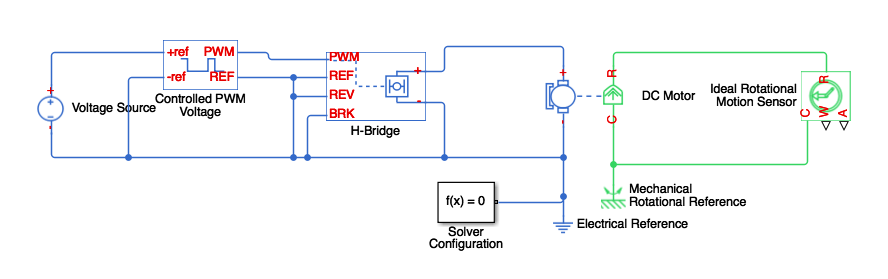
\includegraphics[width=0.8\textwidth]{circuit_simple}
\caption{Ein erster einfacher Antrieb für den Motor ohne Drehzahlregler}
\label{fig:circuit_simple}
\end{center}
\end{figure}

Wichtig hier war dass die HBrücke und der PWM-Regler dasselbe Referenzpotential besitzen und dass ein 'Solver Configuration'-Block mit dem System verbunden ist. Dieser wird benötigt damit Matlab weiss wie er das System ausrechnen soll. Der Motor lief danach wie gewünscht an. Die Simulation dauerte schon für 3 Sekunden Simulationszeit extrem lange. Die Ursache hierfür wurde wie im PWM-Signal wie in Abbildung \ref{fig:pwm} ersichtlich gefunden. Hier müessen natürlich extremkleine Simulationsschritte gemacht werden um das Signal korrekt wiedergeben zu können.
Um das Problem zu beheben wurde der PWM-Mode auf 'Averaged' gestellt, da die HBrücke sich sowieso in diesem Modus befindet.
Nach dieser Optimierung lief die Simulation jeweils in Nullzeit und der Regelkreis konnte ungehindert konstruiert werden.

\begin{figure}
\begin{center}
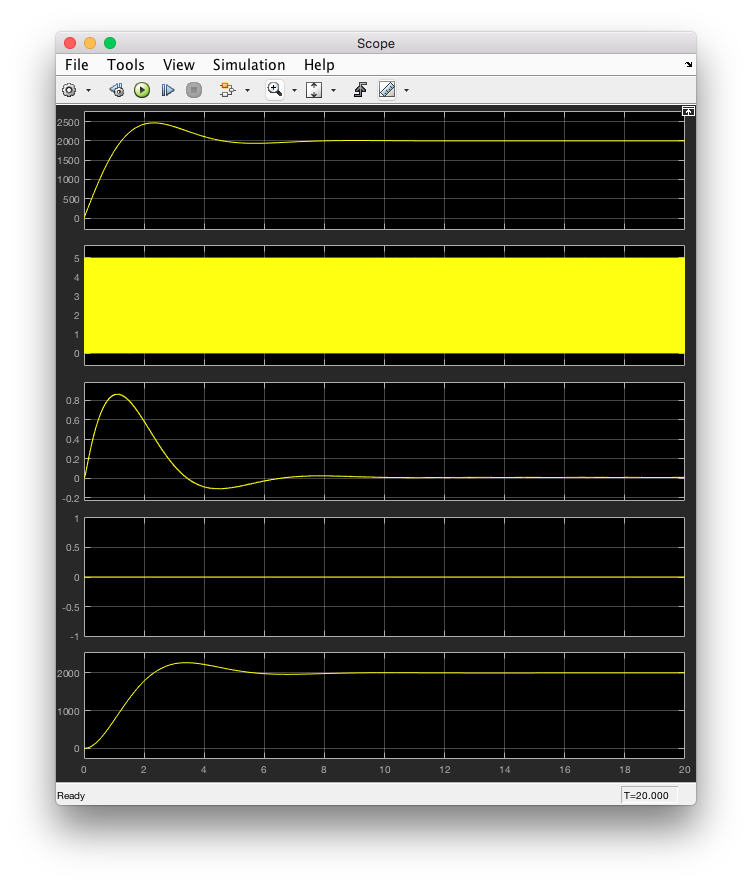
\includegraphics[trim={2cm 18cm 2cm 3.6cm},clip,width=0.8\textwidth]{pwm}
\caption{Das untere Signal zeigt sehr schön wieviele Punkte gerechnet wurden im Vergleich zum oberen Signal.}
\label{fig:pwm}
\end{center}
\end{figure}

In einem nächsten Schritt wurde ein PID-Regler ins System eingefügt. Zudem wurde die Konstantspannungsquelle durch eine verstellbare Spannungsquelle ersetzt.
Dieser Schritt is in Abbildung \ref{fig:pid} zu sehen.

\begin{figure}
\begin{center}
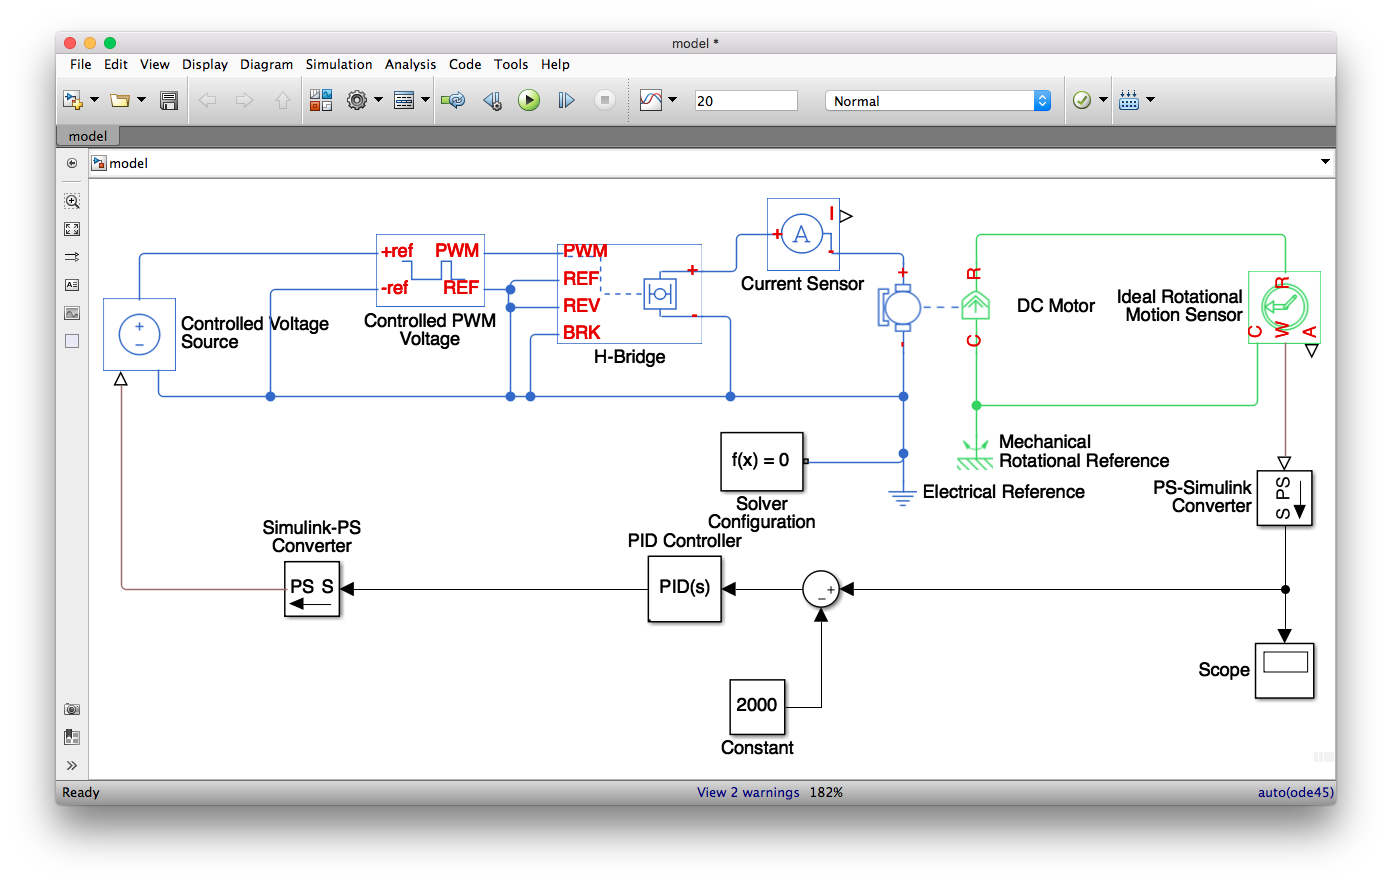
\includegraphics[trim={3.6cm 5.2cm 2.2cm 6.5cm},clip,width=0.8\textwidth]{pid}
\caption{Vollständiger Regelkreis, welcher den Motor auf die gewünschte Drehzahl bringt.}
\label{fig:pid}
\end{center}
\end{figure}

In Abbildung \ref{fig:first_osc} kann die geregelte Drehzahl erkannt werden. Wie man unschwer erkennt oszilliert die Drehzahl extrem stark. Dies deutete auf ein viel zu hohes P hin.
Da der Wertebereich des PWM-Regler-Inputs zwischen 0 und 5 Volt liegt aber der Drehzahl-Output des Motors bei 0 bis 4000 Umdrehungen hat der PID-Regler den PWM-Regler massiv übersteuert.

\begin{figure}
\begin{center}
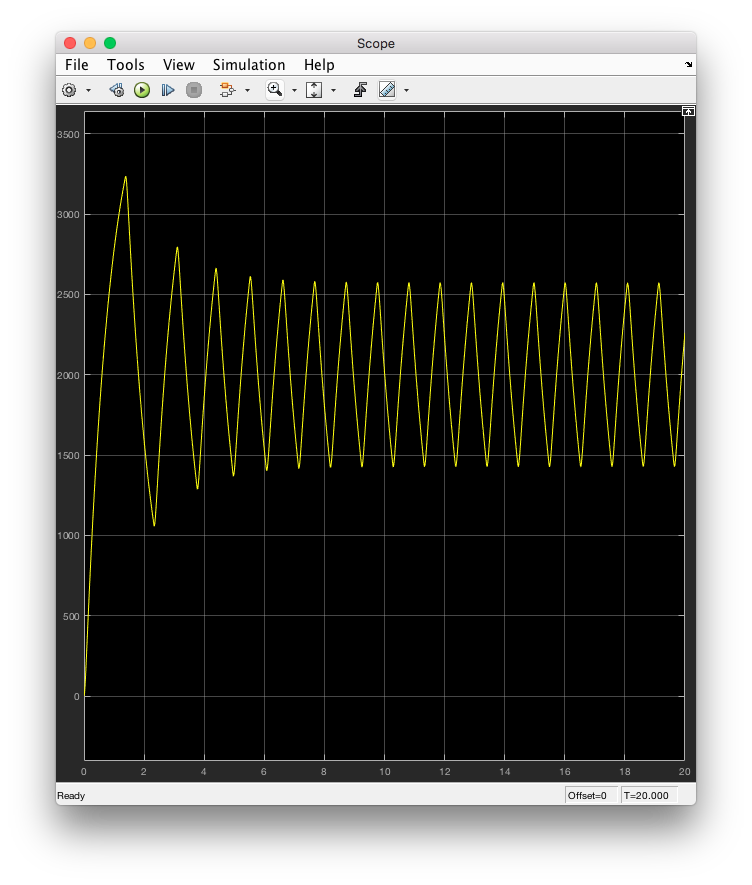
\includegraphics[trim={2cm 8cm 2.2cm 4cm},clip,width=0.8\textwidth]{first_osc}
\caption{Die oszillierende Drehzahl des Motors aufgrund eines ungewollten on-off-Reglers.}
\label{fig:first_osc}
\end{center}
\end{figure}

Dafür wurde dann ein Gain von $\frac{1}{800}$ wie in Abbildung \ref{fig:total} zu sehen in den Regelkreis eingefügt. Zudem wurde der maximale Wertebereich des PID-Reglers auf zwischen 0 und 1 eingestellt um eine Überspannung am PWM-Regler zu vermeiden.

Nun zeigte der Regler schon ein ziemlich gutes Verhalten. In nur 3 Sekunden konnte er von 0 auf stabile 2000 Umdrehungen pro Minute regeln.
Da ein Motor aber sogut wie nie ohne Last verwendet wird, wurde ein Gegenmoment an den Motor angehängt, welches nach einer Totzeit von 2 Sekunden ein Moment von 0.1Nm auf den Motor wirken lässt und ihn belastet.

Dieser finale Regelkreis ist in Abbildung \ref{fig:total} zu erkennen.

\begin{figure}
\begin{center}
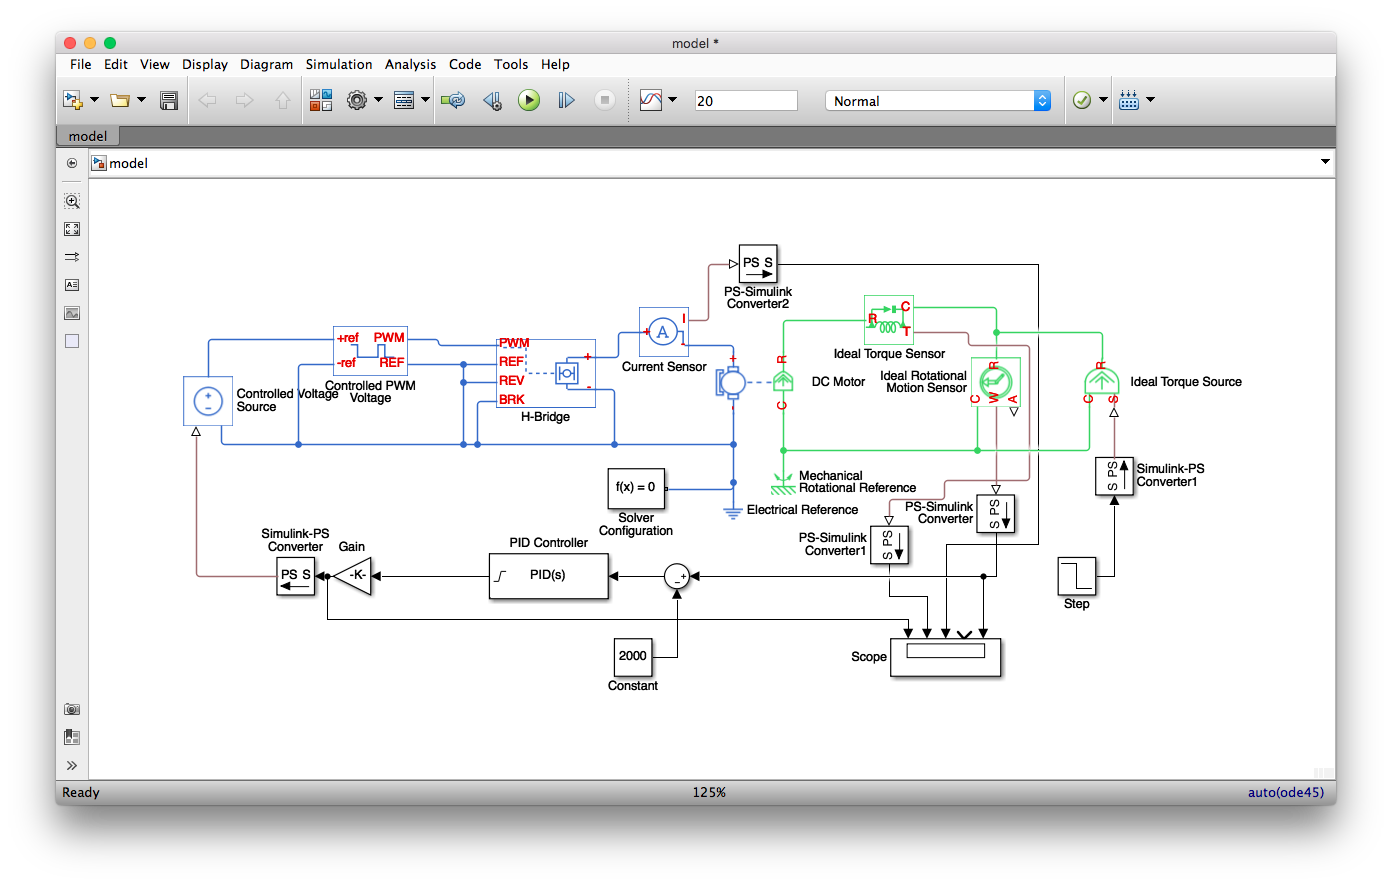
\includegraphics[trim={5cm 6cm 2.2cm 8cm},clip,width=1\textwidth]{total}
\caption{Der komplette Regelkreis mit PID-Regler, korrekt skaliert und einer Last.}
\label{fig:total}
\end{center}
\end{figure}

\section{Ergebnisse}

In Abbildung \ref{fig:no_load} kann man sehr schön erkennen, wie der vollständige PID-Regler einen Motor ohne Last ausregelt. Nach nur 2 Sekunden ist der Regler auf Solldrehzahl und nach 6 Sekunden schön eingeschwungen.
In Abbildung \ref{fig:load} ist das Regelverhalten mit Zuschaltung einer Last ab Sekunde 2 ersichtlich. Man erkennt gut wie der Regler anfängt auf den Sollwert von 2000 Umdrehungen pro Minute zu regeln. Nach zwei Sekunden gibt es einen Einbruch nach unten, da dort das Drehmoment anfängt entgegenzuwirken. Danach erholt sich der Regler schön und erreicht nach 6 Sekunden den Sollwert.
Die Kurven zeigen der Reihe nach die Kontrollspannung am PWM-Regler, das auf den Motor wirkende Drehmoment, den vom Motor aufgenommenen Strom und zunterst die Drehzahl des Motors.

Der Regler ist nicht optimal eingestellt und sollte sicherlich nicht so einen starken Hit erfahren wenn das Drehmoment einsetzt. Zudem könnte er Anfangs wahrscheinlich noch agressiver nach oben regeln.
Dies zu tunen wurde mit dem Tuning-Tool von Simulink versucht, jedoch kann das Tool aufgrund der verschiedenen Systeme und nichtlinearen Komponenten den Kreis nicht linearisieren und so die Koeffizienten nicht bestimmen.
Dies wäre für einen weiterführenden Versuch sicherlich spannend, Zweck dieser übung war jedoch nicht der perfekte Regler, weswegen dieser nicht weiter getunt wurde.

\begin{figure}
\begin{center}
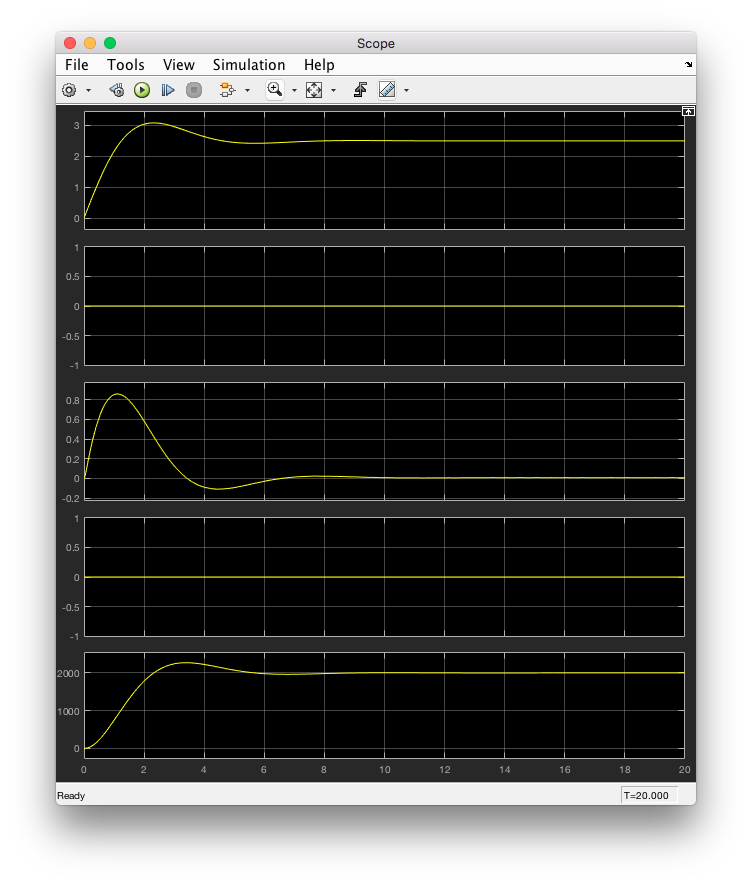
\includegraphics[trim={2cm 3cm 2.2cm 3.7cm},clip,width=0.5\textwidth]{scope_no_load}
\caption{Verhalten des vollständigen Regelkreises ohne Last.}
\label{fig:no_load}
\end{center}
\end{figure}

\begin{figure}
\begin{center}
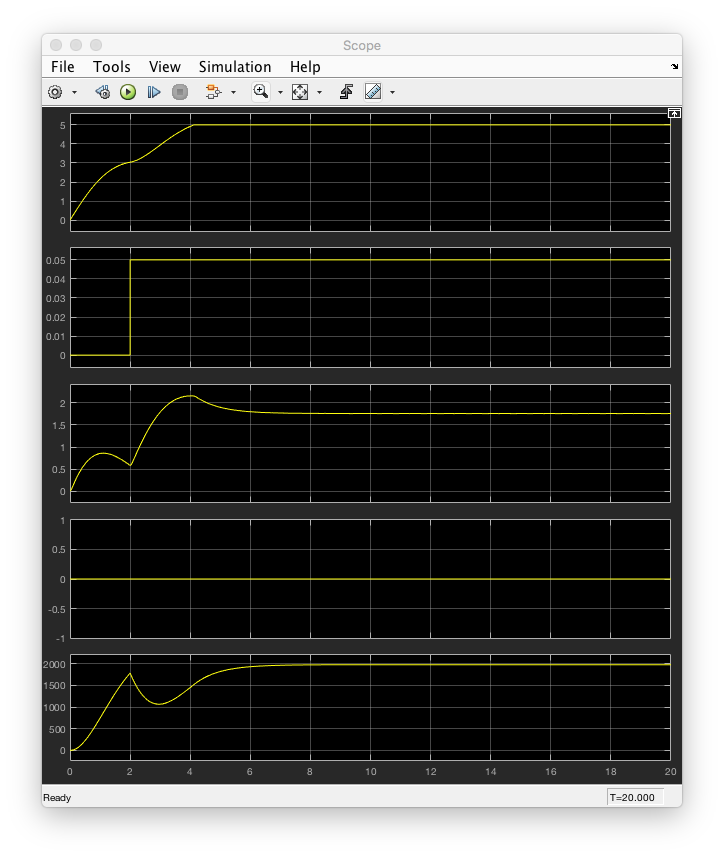
\includegraphics[trim={1.5cm 2.8cm 1.5cm 3.9cm},clip,width=0.5\textwidth]{scope_load}
\caption{Verhalten des vollständigen Regelkreises unter Last ab Sekunde 2.}
\label{fig:load}
\end{center}
\end{figure}

\section{Zusammenfassung}

Der Versuch hat die erweiterten Möglichkeiten von Simulink/Simscape nahe gebracht. Natürlich könnte man hier noch viel weiter gehen. Bisher haben wir nur mit Simulink in der mathematischen Domäne gearbeitet, was gewisse Dinge vereinfacht, wie zum Beispiel dass man ein System einfahc durch eine Matlab-Funktion ersetzen kann ohne sich um die physikalischen Schnittstellen kümmern zu müssen.
Um die physikalische Korrektheit zu verifizieren ist dann aber das physikalische Modell von grossem Vorteil.
Sehr positiv überrascht hat uns dass Simscape so perfekt mit den korrekten Einheiten rechnen kann, diese umrechnet und kontrolliert.

Alles in allem war der Versuch spannend und hat wieder einmal die Matlab-Kenntnisse aufgefrischt.

\end{document}

